% Policy figure, panel (a): where ODRL policies attach in a converted graph.
% Drawn from the VCF-RDFizer policy demonstrator's example (examples/policy/policy.ttl,
% ecrum19/VCF-RDFizer#26): one participant's consent on their file, and the two
% cohort rules on a region selection and a variant selection.
% Standalone TikZ source; build with: pdflatex fig-policy-attach.tex -> fig-policy-attach.pdf
% Drawn at the journal text width (372pt, about 13.1 cm) so it is included unscaled.
\documentclass[border=2pt]{standalone}
\usepackage[T1]{fontenc}
\usepackage{helvet}
\renewcommand{\familydefault}{\sfdefault}
\usepackage{tikz}
\usetikzlibrary{arrows.meta,positioning,calc}

% Figure 2's palette for data classes, plus one hue for policy.
\definecolor{crec}{HTML}{DDEFEF}  \definecolor{crecd}{HTML}{1F7F83}
\definecolor{cfile}{HTML}{F6E3B4} \definecolor{cfiled}{HTML}{C9A227}
\definecolor{csel}{HTML}{F2F2F0}  \definecolor{cseld}{HTML}{6E6D68}
\definecolor{cpol}{HTML}{E8E4F7}  \definecolor{cpold}{HTML}{4A3AA7}

\newcommand{\head}{\bfseries}

\begin{document}
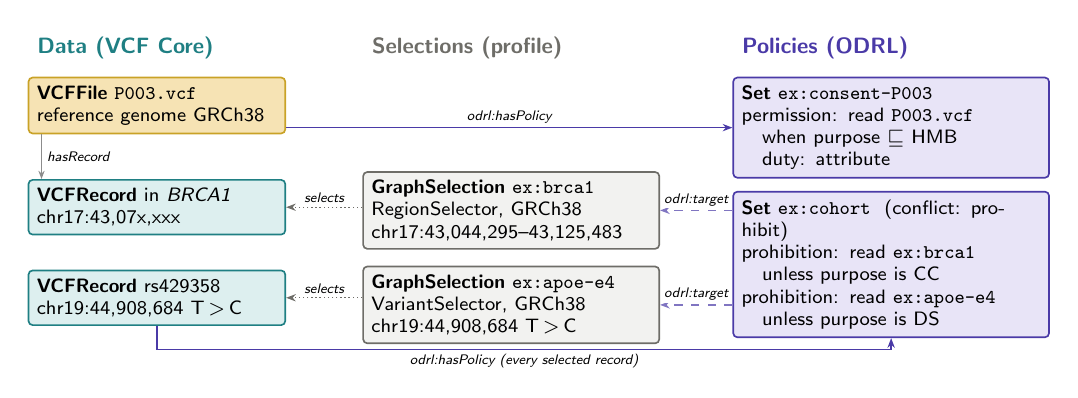
\begin{tikzpicture}[
  font=\scriptsize,
  box/.style={draw, rounded corners=1.5pt, line width=0.6pt, align=left, inner sep=3pt,
              text width=#1, anchor=north west},
  lane/.style={font=\footnotesize\bfseries\itshape, anchor=south west},
  link/.style={-{Stealth[length=3.5pt]}, line width=0.6pt, draw=cpold},
  target/.style={-{Stealth[length=3.5pt]}, line width=0.5pt, draw=cpold!70, dashed},
  selects/.style={-{Stealth[length=3.5pt]}, line width=0.5pt, draw=cseld, densely dotted},
  data/.style={-{Stealth[length=3pt]}, line width=0.45pt, draw=black!45},
  p/.style={font=\tiny\itshape, fill=white, inner sep=0.8pt},
]

% ------------------------------------------------------------ lanes
\node[lane, text=crecd] at (0,0.1) {Data (VCF Core)};
\node[lane, text=cseld] at (4.25,0.1) {Selections (profile)};
\node[lane, text=cpold] at (8.95,0.1) {Policies (ODRL)};

% ------------------------------------------------------------ data
\node[box=3.05cm, fill=cfile, draw=cfiled] (file) at (0,0) {%
  {\head VCFFile} \texttt{P003.vcf}\\ reference genome GRCh38};
\node[box=3.05cm, fill=crec, draw=crecd] (rec1) at (0,-1.3) {%
  {\head VCFRecord} in \textit{BRCA1}\\ chr17:43{,}07x{,}xxx};
\node[box=3.05cm, fill=crec, draw=crecd] (rec2) at (0,-2.45) {%
  {\head VCFRecord} rs429358\\ chr19:44{,}908{,}684 T\,$>$\,C};
\draw[data] ([xshift=5pt]file.south west) -- node[p, right=1pt]{hasRecord} ([xshift=5pt]rec1.north west);

% ------------------------------------------------------------ selections
\node[box=3.55cm, fill=csel, draw=cseld] (sel1) at (4.25,-1.2) {%
  {\head GraphSelection} \texttt{ex:brca1}\\ RegionSelector, GRCh38\\ chr17:43{,}044{,}295--43{,}125{,}483};
\node[box=3.55cm, fill=csel, draw=cseld] (sel2) at (4.25,-2.4) {%
  {\head GraphSelection} \texttt{ex:apoe-e4}\\ VariantSelector, GRCh38\\ chr19:44{,}908{,}684 T\,$>$\,C};
\draw[selects] (sel1.west |- rec1.east) -- node[p, above=0.5pt]{selects} (rec1.east);
\draw[selects] (sel2.west |- rec2.east) -- node[p, above=0.5pt]{selects} (rec2.east);

% ------------------------------------------------------------ policies
\node[box=3.8cm, fill=cpol, draw=cpold] (consent) at (8.95,0) {%
  {\head Set} \texttt{ex:consent-P003}\\
  permission: read \texttt{P003.vcf}\\
  \quad when purpose $\sqsubseteq$ HMB\\
  \quad duty: attribute};
\node[box=3.8cm, fill=cpol, draw=cpold] (cohort) at (8.95,-1.45) {%
  {\head Set} \texttt{ex:cohort} \ (conflict: prohibit)\\
  prohibition: read \texttt{ex:brca1}\\
  \quad unless purpose is CC\\
  prohibition: read \texttt{ex:apoe-e4}\\
  \quad unless purpose is DS};

% hasPolicy: what `attach` writes into the graph
\draw[link] (file.east |- consent.west) -- node[p, above=0.5pt]{odrl:hasPolicy} (consent.west);
\draw[link] (rec2.south) -- ++(0,-0.3) -| node[p, pos=0.25, below=0.5pt]{odrl:hasPolicy (every selected record)} (cohort.south);
% the rules' targets
\draw[target] (cohort.west |- sel1.east) -- node[p, above=0.5pt]{odrl:target} (sel1.east);
\draw[target] (cohort.west |- sel2.east) -- node[p, above=0.5pt]{odrl:target} (sel2.east);

\end{tikzpicture}
\end{document}
